\begin{figure}[tbp]
\centering
\begin{minipage}[t]{0.43\linewidth}
\centering
\textbf{(a) Projection along a pure run}\par\smallskip
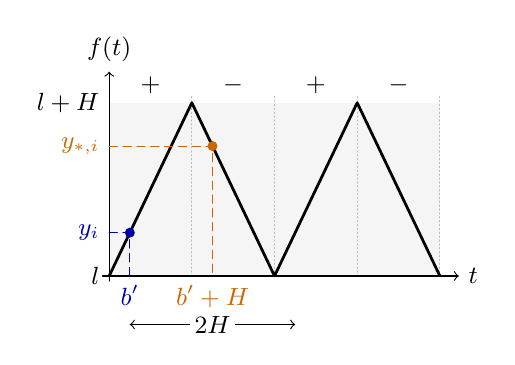
\begin{tikzpicture}[x=1.05cm,y=2.2cm,font=\small,
  line cap=round,line join=round]
  \path[fill=gray!8] (0,0) rectangle (4,1);
  \foreach \x in {0,1,2,3,4}
    \draw[gray!55,densely dotted] (\x,0) -- (\x,1.04);
  \draw[->] (-.08,0) -- (4.23,0) node[right] {$t$};
  \draw[->] (0,-.03) -- (0,1.18) node[above] {$f(t)$};
  \draw[line width=1pt] (0,0) -- (1,1) -- (2,0) -- (3,1) -- (4,0);
  \node[left] at (0,0) {$l$};
  \node[left] at (0,1) {$l+H$};
  \draw[blue!65!black,densely dashed] (0,.25) -- (.25,.25) -- (.25,0);
  \draw[orange!80!black,densely dashed] (0,.75) -- (1.25,.75) -- (1.25,0);
  \fill[blue!65!black] (.25,.25) circle (1.8pt);
  \fill[orange!80!black] (1.25,.75) circle (1.8pt);
  \node[left,text=blue!65!black] at (0,.25) {$y_i$};
  \node[left,text=orange!80!black] at (0,.75) {$y_{*,i}$};
  \node[below,text=blue!65!black] at (.25,0) {$b'$};
  \node[below,text=orange!80!black] at (1.25,0) {$b'+H$};
  \draw[<->] (.25,-.28) -- (2.25,-.28)
    node[midway,fill=white,inner sep=1.5pt] {$2H$};
  \foreach \x/\sign in {.5/+,1.5/-,2.5/+,3.5/-}
    \node at (\x,1.1) {$\sign$};
\end{tikzpicture}
\par\smallskip
{\small
$\displaystyle f(t+H)=2l+H-f(t),$\par
$\displaystyle y_i+y_{*,i}=2l+H.$\par\smallskip
The signs record the alternating\par orientations of successive cells.}
\end{minipage}\hfill
\begin{minipage}[t]{0.54\linewidth}
\centering
\textbf{(b) One successful column}\par\smallskip
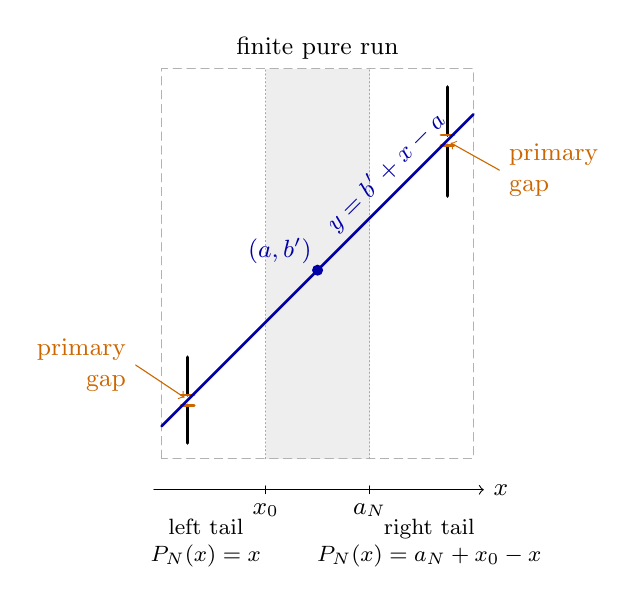
\begin{tikzpicture}[x=.33cm,y=.33cm,font=\small,
  line cap=round,line join=round]
  \path[fill=gray!13] (0,-7) rectangle (4,8);
  \draw[gray!60,densely dashed] (-4,-7) rectangle (8,8);
  \node[above,align=center] at (2,8) {finite pure run};
  \draw[gray!70,densely dotted] (0,-7) -- (0,8);
  \draw[gray!70,densely dotted] (4,-7) -- (4,8);
  \draw[line width=1.3pt] (-3,-6.4) -- (-3,-4.95);
  \draw[line width=1.3pt] (-3,-4.55) -- (-3,-3.1);
  \draw[line width=1.3pt] (7,3.1) -- (7,5.05);
  \draw[line width=1.3pt] (7,5.45) -- (7,7.3);
  \draw[orange!80!black,line width=1pt] (-3.25,-4.95) -- (-2.75,-4.95);
  \draw[orange!80!black,line width=1pt] (-3.25,-4.55) -- (-2.75,-4.55);
  \draw[orange!80!black,line width=1pt] (6.75,5.05) -- (7.25,5.05);
  \draw[orange!80!black,line width=1pt] (6.75,5.45) -- (7.25,5.45);
  \draw[blue!65!black,line width=1pt] (-4,-5.75) -- (8,6.25);
  \fill[blue!65!black] (2,.25) circle (2pt);
  \node[above left,text=blue!65!black,inner sep=2pt] at (2,.25) {$(a,b')$};
  \node[rotate=45,above,text=blue!65!black,inner sep=3pt]
    at (5.2,3.45) {$y=b'+x-a$};
  \draw[orange!80!black,->] (-5,-3.4) -- (-3.12,-4.65);
  \node[left,align=right,text=orange!80!black] at (-5,-3.4)
    {primary\\gap};
  \draw[orange!80!black,->] (9,4.1) -- (7.12,5.15);
  \node[right,align=left,text=orange!80!black] at (9,4.1)
    {primary\\gap};
  \draw[->] (-4.3,-8.2) -- (8.4,-8.2) node[right] {$x$};
  \draw (0,-8.05) -- (0,-8.35) node[below] {$x_0$};
  \draw (4,-8.05) -- (4,-8.35) node[below] {$a_N$};
  \node[align=center,font=\footnotesize] at (-2.3,-10.25)
    {left tail\\$P_N(x)=x$};
  \node[align=center,font=\footnotesize] at (6.3,-10.25)
    {right tail\\$P_N(x)=a_N+x_0-x$};
\end{tikzpicture}
\par\smallskip
{\small
$\displaystyle a\equiv X_*-H+O(\gamma)\pmod{2H}.$\par
Shading marks the central interval, whose image\par
$P_N([x_0,a_N])\subset[x_0-2H,x_0+v]$ is wall-free.}
\end{minipage}
\caption{The two coordinate projections in the final reflection construction.
Write $l=l_i$ and $H=H_i$.
Panel (a) shows the triangular projection to the original marker cell;
shifting a marker ordinate by an odd multiple of $H$ brings its projection
to the anchor height. In panel (b), only the tail-wall portions crossed by
one successful probe line are shown. At either tail wall $x_w$, the
congruence $x_w-a\equiv H+O(\gamma)\pmod{2H}$ places
$f(b'+x_w-a)$ inside a primary gap around $y_{*,i}$. The central
interval has no vertical-wall preimage. The pure run extends beyond the
line's passage through the finite horizontal support, so horizontal
solids are avoided as well. Gap-center crossings and distances are
schematic; the actual $O(\gamma)$ offsets fit within the primary openings.
Secondary gaps make the later fold cuts vacant and are not used for this
diagonal clearance.}
\label{fig:reflection-template-projections}
\end{figure}
